\begin{homeworkProblem}
    \textbf{Pathria Beale (PB) 1.2}

    Assuming that the entropy $S$ and the statistical number $\Omega$ of a physical system are related through an arbitrary functional form
    $$
    S=f(\Omega),
    $$
    show that the additive character of $S$ and the multiplicative character of $\Omega$ necessarily require that the function $f(\Omega)$ be of the form (1.2.6).

    \begin{callout}{Solution:}
    Choice of $S = k_B\ln(\Omega)$ by the fact that it suits the optimization condition well, viewed even as just a mathematical object that I can use elsewhere seems well-justified to me. If I'm to prove that this is the only choice, it is useful to start with
    \begin{align*}
        f(\Omega_A \Omega_B) = f(\Omega_A) + f(\Omega_B)
    \end{align*}

    This is an obvious feature of logarithms, but as it's how I choice the log, I can check how their derivatives act in the general case
    \begin{align*}
        \frac{\partial}{\partial \Omega_A} &\to \Omega_B f'(\Omega_A \Omega_B) = f'(\Omega_A) \\
        \frac{\partial}{\partial \Omega_B} &\to \Omega_A f'(\Omega_A \Omega_B) = f'(\Omega_B)
    \end{align*}

    so, for something like $Af'(AB)=f'(B)$ $f'$ would have to integrate like a logarithm (to cancel with that outside term).

    % Assuming that the entropy $S$ and the statistical number $\Omega$ of a physical system are related through an arbitrary functional form
    % \[
    %     S=f(\Omega),
    % \]
    % show that the additive character of $S$ and the multiplicative character of $\Omega$ necessarily require that the function $f(\Omega)$ be of the form (1.2.6).
    %
    % \begin{callout}{Solution:}
    %
    % I might begin by imagining two systems, A and B, in contact with one another. Because the probability of finding the combined system in a particular state is the product of finding the two systems in corresponding states, their total multiplicity must also be the product of the multiplicity of both systems:
    % $$\Omega_{total} = \Omega_A \Omega_B$$
    %
    % The most probable macrostate corresponds to a maxima in $\Omega_{total}$, such that:
    % \begin{align*}
    %     d \Omega_{total} &= (d \Omega_A)\Omega_B + \Omega_A(d \Omega_B) = 0 \\ 
    %     \frac{d \Omega_{total}}{\Omega_{total}} &= \frac{(d \Omega_A)\Omega_B}{\Omega_{total}} + \frac{\Omega_A(d \Omega_B)}{\Omega_{total}} = 0 \\ 
    %      &= \frac{d \Omega_A}{\Omega_{A}} + \frac{d \Omega_B}{\Omega_{B}} = 0
    % \end{align*}
    %
    % If I are defining entropy as a quantity that is additive and at an extremum for a system to be at equilibrium, I must express this with a logarithm
    % $$d(\ln(\Omega_{total})) = d(\ln_{\Omega_A} + d(\ln_{\Omega_B} = 0$$
    %
    % Such that 
    % $$dS_{total} = dS_A + dS_B = 0$$

    \end{callout}

\end{homeworkProblem}

\newpage
\begin{homeworkProblem}
    \textbf{Pathria Beale (PB) 1.4}

    In a classical gas of hard spheres (of diameter $D$), the spatial distribution of the particles is no longer uncorrelated. Roughly speaking, the presence of $n$ particles in the system leaves only a volume $(V-nv_0)$ available for the $(n+1)$th particle; clearly, you would be proportional to $nv_0$. Assuming that $Nv_0\ll V$, determine the dependence of $\Omega(V,E,N)$ on $V$ (compare to equation (1.4.1)) and show that, as a result of this, $V$ in the ideal-gas law (1.4.3) gets replaced by $(V-b)$, where $b$ is four times the actual volume occupied by the particles.

    \begin{callout}{Solution:}

    I could write the volume of each particle as:
    $$v_{0}= \frac{4}{3} \pi (D/2)^{3}$$

    But! The volume accessible to each particle is very much not 
    $$V-nv_{0}$$

    Since that would imply the configuraion shown in 1.4a is correct. Two spheres can't overlap like this, so the distance between their centers has to be separated by D (1.4b)
    $$\frac{D}{2}+\frac{D}{2}=D$$

    This is eight times the particle's radius, since:
    $$\text{excluded volume} = \frac{4}{3} \pi (2*D/2)^{3} = 8 * \underbrace{\frac{4}{3} \pi (D/2)^{3}}_{=v_{0}}$$

    % To avoid double counting, this is halved, since particle $n$ excludes particle $n+1$ the same way particle $n+1$ excludes particle $n$. Thus, the volume excluded by the $n$-th particle is

    Or more compactly,
    $$\text{accessible volume for particle $n+1$} = V-8nv_{0}$$

    I spent a solid hour wondering why this is twice as much as it seemingly should be but the problem is asking for the ideal gas law so I can follow that derivation. We'll need the entropy,
    \begin{align*}
        \Omega &= \prod_{n=0}^{N-1} (V-8nv_{0}) = (V)(V-8v_{0})(V-16v_{0})\dots \\ 
        S &= \ln \left( \prod_{n=0}^{N-1} (V-8nv_{0}) \right) = \ln(V)\ln(V-8v_{0})\ln(V-16v_{0})\dots \\ 
        &= N\ln(V) + \sum_{n=1}^{N-1} \ln \left( 1-\frac{8nv_{0}}{V} \right) \\
        &\approx N\ln(V) + \sum_{n=1}^{N-1} \left( -\frac{8nv_{0}}{V} \right) \\
        &\approx N\ln(V) -\frac{8N^{2}v_{0}}{2V} \\
    \end{align*}

    The next step of the derivation had
    \begin{align*}
        \frac{P}{T} = k_B \left( \frac{\partial S}{\partial V} \right)_{N,E} = \frac{Nk_B}{V} + \frac{4N^{2}k_B v_{0}}{V}
    \end{align*}

    And so the gas law becomes 
    \begin{align*}
        PV = Nk_BT\left( 1 + 4v_{0} \right) \\
        \boxed{PV-4Nk_BTv_{0} = Nk_BT} 
    \end{align*}


\begin{figure}[H]
  \centering
  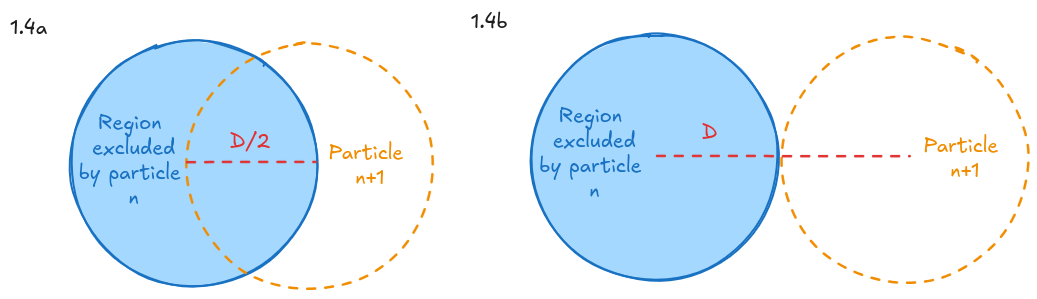
\includegraphics[width=0.8\textwidth]{../assets/1.4-Fig1.png}
  \label{fig:1.4-fig1}
\end{figure}

    \end{callout}

\end{homeworkProblem}

\newpage
\begin{homeworkProblem}
    \textbf{Pathria Beale (PB) 1.7}

    Study the statistical mechanics of an extreme relativistic gas characterized by the
    single-particle energy states
    \[
        \epsilon(n_x,n_y,n_z)
        =
        \frac{hc}{2L}
        \left(n_x^2+n_y^2+n_z^2\right)^{1/2},
    \]
    instead of (1.4.5), along the lines followed in Section 1.4. Show that the ratio
    $C_P/C_V$ in this case is $4/3$, instead of $5/3$.

    \begin{callout}{Solution:}

        (1.4.5) states:
        $$ \varepsilon\left(n_x, n_y, n_z\right)=\frac{h^2}{8 m L^2}\left(n_x^2+n_y^2+n_z^2\right) ; \quad n_x, n_y, n_z=1,2,3, \ldots $$

        This is like saying that the radius of accessible energies in phase space is smaller? $L$ is also of a reduced dimension. I would say the number of microstates is the number of different choices of $n_r$, i.e.:
        \begin{align*}
            \frac{2\cancelto{V^{{1} / {3}}}{L}\epsilon}{hc} &= \left(n_x^2+n_y^2+n_z^2\right)^{1 / 2} = \epsilon^{*} \\ 
            \sum_{r=1}^{3N} n_r &= \left( \frac{2V^{{1} / {3}}{L}E}{hc} \right) = E^{*}
        \end{align*}

        And from this I should expect $\Omega \equiv \Omega(N, V^{N}, E^{3N})$.

        \begin{align*}
            S &= k_B \left( \ln f(N) + N \ln V + 3N \ln E \right) \\
            \frac{1}{T} &= \left( \frac{\partial S}{\partial E} \right)_{P,V} = \frac{3Nk_B}{E} \implies E=3Nk_BT \\
            P &= T\left( \frac{\partial S}{\partial V} \right)_{N,E} = \frac{Nk_BT}{V}
        \end{align*}

        \begin{align*}
            C_V &\equiv \left( \frac{\partial E}{\partial T} \right)_{N,V} = 3Nk_B\\
            C_P &\equiv \left( \frac{\partial (E+PT)}{\partial T} \right)_{E,V} = 3Nk_B + Nk_B\\
        \end{align*}

        \begin{align*}
            \boxed{\frac{C_P}{C_V} =\frac{4 Nk_B}{3 Nk_B} = \frac{4}{3}
}
        \end{align*}

    \end{callout}

\end{homeworkProblem}

\newpage
\begin{homeworkProblem}
    \textbf{Pathria Beale (PB) 2.1}

    Show that the volume element
    \[
        d\omega=\prod_{i=1}^{3N}(dq_i\,dp_i)
    \]
    of the phase space remains invariant under a canonical transformation of the
    (generalized) coordinates $(q_i,p_i)$ to any other set of (generalized) coordinates
    $(Q_i,P_i)$.

    \textit{Hint:} Before considering the most general transformation of this kind, which is referred to as a contact transformation, it may be helpful to consider a point transformation---one in which the new coordinates $Q_i$ and the old coordinates $q_i$ transform only among themselves.

    \begin{callout}{Solution:}

        A useful resource for canonical transformations: \href{https://phys.libretexts.org/Bookshelves/Classical_Mechanics/Variational_Principles_in_Classical_Mechanics_%28Cline%29/15%3A_Advanced_Hamiltonian_Mechanics/15.03%3A_Canonical_Transformations_in_Hamiltonian_Mechanics}{link}

        The approach I will attempt is to express what a canonical transformation is, find an expression to relate my variables before and after the transformation, then take the jacobian which will be 1 if and only if they are invariant under a point transformation.
 
        A transformation is canonical when Hamilton's equations are not changed by it. More precisely,
    $$\sum_i p_i dq_i - \sum_i P_i dQ_i = dF$$

    Where $F$ is a generating function, and can be of four forms:
    \begin{align*}
        F_1(\mathbf{q}, \mathbf{Q}, t) \\
        F_{2}(\mathbf{q}, \mathbf{P}, t) - \mathbf{Q}\cdot \mathbf{P} \\
        F_3(\mathbf{p}, \mathbf{Q}, t) + \mathbf{q}\cdot \mathbf{p} \\
        F_{4}(\mathbf{p}, \mathbf{P}, t) + \mathbf{q}\cdot \mathbf{p} - \mathbf{Q}\cdot \mathbf{P}
    \end{align*}

    I can try choosing a $F$ which is of the \textit{old} coordinates and \textit{new} momenta. This is $F_{2}$ and might look like 
    \begin{align*}
        F_{2} = \sum_i \mathbf{P}_i \mathbf{Q}_i(q)        
    \end{align*}

    And because it is of type $F_{2}$,
    \begin{align*}
        \mathbf{p} = \frac{\partial F_{2}}{\partial \mathbf{q}} \qquad \mathbf{Q} = \frac{\partial F_{2}}{\partial \mathbf{P}}
    \end{align*}

    If I were to try to express $\mathbf{p}_i$ now
    \begin{align*}
        \mathbf{p}_i &= \frac{\partial}{\partial \mathbf{q}_i} \sum_j \mathbf{P}_j \mathbf{Q}_j(\mathbf{q}_i) \\ 
                     &= \sum_j \mathbf{P}_j \frac{\partial \mathbf{Q}_j}{\partial \mathbf{q}_i}
    \end{align*}

    I'd like to try a different setup to see what happens. If I choose a type $F_{3}$ generating function,
    \begin{align*}
        \mathbf{q} = -\frac{\partial F_{3}}{\partial \mathbf{p}} \qquad \mathbf{P} = -\frac{\partial F_{3}}{\partial \mathbf{Q}}
    \end{align*}

    Something like this could be a suitable $F_{3}$
    \begin{align*}
        F_{3} = -\sum_j \mathbf{p}_j \mathbf{q}_j(\mathbf{Q})        
    \end{align*}

    And we'd get 
    \begin{align*}
        \mathbf{P}_i &= \frac{\partial}{\partial \mathbf{Q}} \sum_j \mathbf{p}_j \mathbf{q}_j(\mathbf{Q}) \\
        &= \sum_j \mathbf{p}_j  \frac{\partial \mathbf{q}_j(\mathbf{Q})}{\partial \mathbf{Q}}
    \end{align*}

    Which is the inverse relation, and it shows how $\mathbf{P}$ transforms to $\mathbf{p}$! Returning to this problem of proving that point transformations are invariant, the Jacobian is the next natural step
    \begin{align*}
        \frac{\partial (x,y)}{\partial (u,v)} = \left|\begin{matrix} \frac{\partial x}{\partial u} & \frac{\partial x}{\partial v} \\ \frac{\partial y}{\partial u} & \frac{\partial y}{\partial v} \end{matrix}\right|
    \end{align*}

    I could check this quantity, 
    \begin{align*}
        \frac{\partial (q,p)}{\partial (Q,P)} &= \left|\begin{matrix} \frac{\partial q}{\partial Q} & \frac{\partial q}{\partial P} \\ \frac{\partial p}{\partial Q} & \frac{\partial p}{\partial P} \end{matrix}\right| \\
                                              &= \left|\begin{matrix} \frac{\partial q}{\partial Q} & 0 \\ \frac{\partial p}{\partial Q} & \frac{\partial p}{\partial P} \end{matrix}\right| \qquad \text{(See note below)} \\
        &= \frac{\partial q}{\partial Q} \frac{\partial p}{\partial P} \\ 
        &= \frac{\partial q}{\partial Q} \frac{\partial Q}{\partial q} \qquad\text{(Derivative of my eqn. for $p$)} \\ 
        &= 1
    \end{align*}
    Note that $q$ is independent of $P$, but $p$ is dependent on $Q$, since $F_{2}\equiv F_{2}(q,P)$ since old coordinates and new momenta were selected. I would expect that the same result can be achieved with $F_{3}$, it's just going the other way.

    Google tells me that contact transformations built up from infinitesimal point tranformations:
    \begin{align*}
        Q = q + \epsilon \frac{\partial G}{\partial p}, \qquad P = p + \epsilon \frac{\partial G}{\partial q}
    \end{align*}

    The challenge is again to write a Jacobian. I'll need the derivatives (going the other direction, this time):
    \begin{align*}
        \frac{\partial Q_j}{\partial q_j} &= \frac{\partial}{\partial q_j} \left( q_i  + \epsilon \frac{\partial G}{\partial p_i} \right) = 
        \delta_{ij} + \epsilon \frac{\partial^{2}G}{\partial p_i \partial q_j} 
        \\
        \frac{\partial P_j}{\partial q_j} &= \frac{\partial}{\partial q_j} \left( p_i  + \epsilon \frac{\partial G}{\partial q_i} \right) = 
        \epsilon \frac{\partial^{2}G}{\partial q_i \partial p_j} 
        \\
        \frac{\partial Q_j}{\partial p_j} &= \frac{\partial}{\partial p_j} \left( q_i  + \epsilon \frac{\partial G}{\partial p_i} \right) = 
        \delta_{ij} + \epsilon \frac{\partial^{2}G}{\partial p_i \partial p_j} 
        \\
        \frac{\partial P_j}{\partial p_j} &= \frac{\partial}{\partial p_j} \left( p_i  + \epsilon \frac{\partial G}{\partial q_i} \right) = 
        \epsilon \frac{\partial^{2}G}{\partial q_j \partial q_i} 
        \\
    \end{align*}

    So the jacobian is
    \begin{align*}
        \left|\begin{matrix}
            \delta_{ij} + \epsilon \frac{\partial^{2}G}{\partial p_i \partial q_j} &
            \epsilon \frac{\partial^{2}G}{\partial p_i \partial p_j} \\
            \epsilon \frac{\partial^{2}G}{\partial q_j \partial q_i} &
            \delta_{ij} + \epsilon \frac{\partial^{2}G}{\partial q_i \partial p_j}
        \end{matrix}\right|
    \end{align*}

    Which clearly goes to identity for small $\epsilon$.

    \end{callout}

\end{homeworkProblem}

\begin{homeworkProblem}
    \textbf{Pathria Beale (PB) 2.3}

    Starting with the line of zero energy and working in the (two-dimensional) phase space of a classical rotator, draw lines of constant energy that divide phase space into cells of ``volume'' $h$. Calculate the energies of these states and compare them with the energy eigenvalues of the corresponding quantum-mechanical rotator.
    \begin{callout}{Solution:}

    A rigid planar rotator has hamiltonian:
    \begin{align*}
        H(\phi, p_\phi) = \frac{p^{2}_\phi}{2I}
    \end{align*}

    Meanwhile the quantum rotator has the following schrodinger equation and eigenstates/values:
    \begin{align*}
        - \frac{\hbar^{2}}{2I} \frac{\partial^{2} \phi}{\partial \phi^{2}} = E_m^{QM}\psi, 
        \qquad \phi_m = \frac{1}{\sqrt{2\pi}} e^{im\phi}, 
        \qquad E_m^{QM} = \frac{m^{2}\hbar^{2}}{2I}, 
        \qquad m=0,\pm1,\pm2,\dots
    \end{align*}

    These are of a similar form, just with a quantized $p_\phi$. Hamilton's equations read:
    \begin{align*}
        \dot{\phi} &= \frac{\partial H}{\partial p_\phi} = \frac{p_\phi}{I} \\
        \dot{p_\phi} &= -\frac{\partial H}{\partial \phi} = 0 \implies p_\phi = \text{const}
    \end{align*}

    I think this is saying that $\phi$ can take on any value but $p_\phi$ must be the same value regardless of $\phi$. I think that's sensible since I have a spinning rod that never stops due to conservation laws, obviously it will pass through all $\phi$ for any given $p_\phi$. In phase space this is like:

\begin{figure}[H]
  \centering
  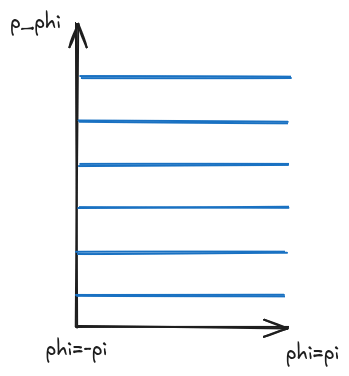
\includegraphics[width=0.3\textwidth]{../assets/H1P5F1.png}
\end{figure}

    If we're letting the volume be $h$, I could write it as something like:
    \begin{align*}
        h = \frac{2\pi}{m}
    \end{align*}

    Since the x-axis of phase space in that picture spans $\phi \in [0,2\pi)$ and I could let the spacing between them be any number $m$. All of those states together should be the observable, so the rotator would take on states like 
    \begin{align*}
        \dots,\, -3h,\, -2h,\, -h,\, 0,\, h,\, 2h,\, 3h,\, \dots
    \end{align*}

    and if I stuck in $p_\phi \to 2\pi / m$, and rearranged, then we'd get the quantum state where $m$ is selecting the energy level (same idea as n-th spacing).

    \end{callout}

\end{homeworkProblem}

\newpage
\begin{homeworkProblem}
    \textbf{Pathria Beale (PB) 2.4}

    By evaluating the "volume" of the relevant region of its phase space, show that
    the number of microstates available to a rigid rotator with angular momentum
    $M$ is $(M/\hbar)^2$. Hence determine the number of microstates that may be
    associated with the quantized angular momentum
    \[
        M_j=\sqrt{j(j+1)}\hbar,
    \]
    where $j=0,\frac{1}{2},1,\frac{3}{2},2,\ldots$, and interpret the result physically.

    \textit{Hint:} It simplifies to consider motion in the variables $\theta$ and $\phi$,
    with
    \[
        M^2=p_\theta^2+\frac{p_\phi^2}{\sin^2\theta}.
    \]
    \begin{callout}{Solution:}

        % Last problem was 2D, this is 3D. We'd just be looking for $\Omega$ or $S$ corresponding to a particular angular momentum. I think in principle it is possible to approach this with a partition function or something, but working it out in phase space is probably easiest since I have a hamiltonian.

       I'll want to check $M$ for practice. The lagrangian is purely kinetic energy:
        \begin{align*}
            L=\frac{1}{2}I (\dot{\theta}^{2} + \dot{\phi}^{2}\sin^{2}\theta)
        \end{align*}

        The Legendre transformation would go like:
        \begin{align*}
            p_\theta &= \frac{\partial L}{\partial \dot{\theta}} = I\dot{\theta} &&\implies \dot{\theta} = \frac{p_\theta}{I} \\ 
            p_\phi &= \frac{\partial L}{\partial \dot{\phi}} = I \sin^{2}\theta \dot{\phi} &&\implies \dot{\phi} = \frac{p_\phi}{I \sin^{2}\theta}
        \end{align*}

        Then,
        \begin{align*}
            H &= p_\theta \dot{\theta} + p_\phi \dot{\phi} - L \\
            &= p_\theta\left(\frac{p_\theta}{I}\right)+p_\phi\left(\frac{p_\phi}{I \sin ^2 \theta}\right)-\frac{1}{2} I\left[\left(\frac{p_\theta}{I}\right)^2+\sin ^2 \theta\left(\frac{p_\phi}{I \sin ^2 \theta}\right)^2\right] \\
&=\frac{1}{2 I}\left(p_\theta^2+\frac{p_\phi^2}{\sin ^2 \theta}\right) = \frac{1}{2I} M^{2}
        \end{align*}

        The volume of phase space is reached by integrating over the radius of accessible states. A quick note about the bounds, I shall say there is a maximum $M$ such that $p_\theta^2 + p_\phi^2 \leq M^2$, and it follows that $dp_\theta + dp_\phi = dM$.
        \begin{align*}
            \Gamma &= \int_{0}^{\pi} d\theta \int_{0}^{2\pi} d\phi \iint_{p_\theta^{2} + \frac{p_\phi^{2}}{\sin^{2}\theta \leq M^{2}}} dM
        \end{align*}
        I will let the double integral be the area $A(p_\theta, p_\phi)$ which I sweep over the other dimensions. This follows a standard integral over the area of an ellipse,
        \begin{align*}
            A &= \iint_{p_\theta^{2} + \frac{p_\phi^{2}}{\sin^{2}\theta \leq M^{2}}} dM \\
              &= \sin\theta\iint_{u^{2} + v^{2}\leq M^{2}} du\,dv 
              &\begin{matrix} 
                  u=p_\theta, &v=\frac{p_\phi}{\sin\theta} \\
                  du=dp_\theta, &dv=\frac{dp_\phi}{\sin\theta} 
              \end{matrix} \\
              &= \sin \theta \int_{0}^{2\pi} \,d\alpha \int_{0}^{M} r\, dr \\
              &= \pi M^{2}\sin \theta 
        \end{align*}

        And the rest evaluates simply,
        \begin{align*}
            \Gamma &= \pi M^{2} \int_{0}^{\pi} \sin \theta \,d\theta \int_{0}^{2\pi}  \,d\phi \\
            &= 4\pi^{2}M^{2}
        \end{align*}

        Since the problem is 3D instead of 2D, I could extend the logic from the last problem to be like $h^{N+1}=V$, $N$ being the dimension, which in this case gives us the desired
        \begin{align*}
            \Gamma = \left( \frac{M}{\hbar} \right)^{2}
        \end{align*}

        This was a bit unclear to me but I believe this last part is asking to have us count the number of microstates associated with the $j$-th state alone, and not the sum of states below it. I can look at the difference between the $j$-th and $j-1$-th state:
        \begin{align*}
            \text{number of states} = \left(\frac{M_j}{\hbar}\right)^2 - \left(\frac{M_{j-1}}{\hbar}\right)^2 = j(j+1) - (j-1)j = 2j
        \end{align*}

        Which is off by one compared to the quantum mechanical solution. Perhaps this is sort of like not considering the case that two particles can be in the exact same state at all? Fermion counting rule is minus one and boson is plus one - maybe?

    \end{callout}

\end{homeworkProblem}

\begin{homeworkProblem}
    \textbf{Pathria Beale (PB) 2.7}

    Derive (i) an \emph{asymptotic} expression for the number of ways in which a given
    energy $E$ can be distributed among a set of $N$ one-dimensional harmonic
    oscillators, the energy eigenvalues of the oscillators being
    \[
        \left(n+\frac{1}{2}\right)\hbar\omega;
        \qquad n=0,1,2,\ldots,
    \]
    and (ii) the corresponding expression for the ``volume'' of the relevant region of
    the phase space of this system. Establish the correspondence between the two
    results, showing that the conversion factor $\omega_0$ is precisely $h^N$.
    \begin{callout}{Solution:}

    \begin{enumerate}[(i)]
    \item From a purely counting perspective, the number of ways to distribute $N$ harmonic oscillators is like treating every $n$ as an energy bin for which $N$ particles could sit in. There being no restriction on how many particles can go in each bin means I have a boson-like counting rule. This is a familiar result that's not restricted to the harmonic oscillator - theorem 2: \url{https://en.wikipedia.org/wiki/Stars_and_bars_(combinatorics)}.

        Result of this is:
        $$\Gamma = \begin{pmatrix} n+k-1 \\ k-1 \end{pmatrix}$$

        Confusing notation here since I label energy $n$ --- This would treat $n$ as the energy and $k$ as particle $k= 1, 2, 3, \dots, N$.


        \item Hamiltonian for the classical harmonic oscillator is:
            \begin{align*}
                L &= \frac{1}{2} m\dot{x}^{2} - \frac{1}{2}kx^{2} \quad\to\quad H=\frac{p_x^{2}}{2m} + \frac{1}{2}\omega^{2} x^{2}, \quad \omega=\sqrt{\frac{k}{m}}
            \end{align*}

            We'll again say there's a max energy of $M$, and try to convert this to a polar representation (given the sum of squares) and integrate:
            \begin{align*}
                \Gamma &= \iint_{\frac{p_x^{2}}{2m} + \frac{1}{2}m\omega^{2} x^{2} \leq M} dp_x\,dx \\
                       &= \frac{2}{\omega} \iint_{u^{2}+v^{2} \leq M}^{} \,du\,dv 
                       &\begin{matrix}
                           u = \frac{p_x}{\sqrt{2m}},& v=\frac{\omega x}{\sqrt{2}} \\ 
                           du = \frac{dp_x}{\sqrt{2m}}, & dv= \frac{\omega dx}{\sqrt{2}}
                       \end{matrix} \\
                       &= \frac{1}{\omega} \int_{0}^{2\pi} d \alpha \int_{0}^{\sqrt{M}} r \,dr & 
                       \begin{matrix}
                           u \to r \cos \alpha, & v \to r \sin \alpha
                       \end{matrix} \\ 
                       &= \frac{2\pi M}{\omega}
            \end{align*}

            If we're dividing by $h$ per dimension:
            \begin{align*}
                \Gamma &= \frac{M}{\hbar \omega} = n + \frac{1}{2}
            \end{align*}

            Paying close attention to chapter 1.6, I believe I can extend this to $N$ particles such that:
            \begin{align*}
                \Gamma = \frac{1}{N!} \left( \frac{M}{\hbar \omega} \right)^{N}
            \end{align*}

            Because I have a boson counting rule and I need to avoid double counting since particles are indistinguishable and particle 1 and 2 in the same energy $\epsilon$ is the same as saying particle 2 and 1 in the same energy $\epsilon$, if that makes sense?

    \end{enumerate}

    \end{callout}

\end{homeworkProblem}

\newpage
\begin{homeworkProblem}
    \textbf{(Stirling Formula)}

    In the lecture notes I discussed the Stirling Approximation,
    \[
        n! \approx \sqrt{2\pi n}e^{-n}n^n
        \left\{
            1+\frac{1}{12n}
            +O\left(\frac{1}{n^2}\right)
        \right\}.
    \]

    In particular, I derived the leading order term in the expansion.

    \begin{enumerate}
        \item[(a)] Extend the argument presented in lecture to evaluate the next term in the approximation, i.e., show that it is indeed given by
            \[
                \frac{1}{12n}.
            \]

            \begin{callout}{Solution:}

            This derivation follows our discussion during office hours. Stirling's approximation is for factorials (gamma function). Obviously, if I want to find the next term in an approximation I must be doing some kind of expansion. The gamma function is written as:
            $$\Gamma \equiv \int_{0}^{\infty} dt e^{-t + x \ln t}$$

            substitute $\tau=x\tau$, so that
            \begin{align*}
                \Gamma &= \int_{0}^{\infty} x \,d\tau e^{-x\tau+x\ln(x\tau)} \\
                &= \int_{0}^{\infty} x \,d\tau e^{-x\tau+x\ln x + x\ln \tau} \\
                &= \int_{0}^{\infty} x \,d\tau e^{-x\tau+x\ln \tau} x^{x} \\
                &= \int_{0}^{\infty} x^{x+1} \,d\tau e^{-x(\tau+\ln \tau)} \\
            \end{align*}

            A smart person would inspect their function before expanding it:

\begin{figure}[H]
  \centering
  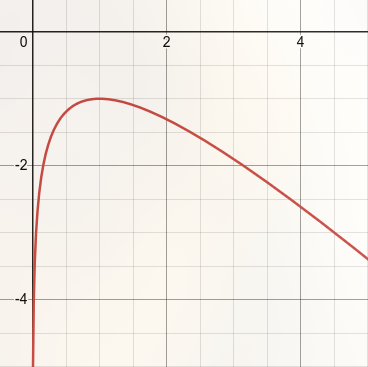
\includegraphics[width=0.5\textwidth]{../assets/1.8-Fig1.png}
  \label{fig:1}
\end{figure}

Notice there is a maxima at $\tau=1$. Because I are integrating this function, it is close to the maxima that most of the contribution will happen. For example, if I were to expand about $\tau=0$, then I would probably not get a very good solution. Even better, I can expand as a perturbation on another function. To handle this, I can choose to introduce $f(\beta(\tau))=-1-\beta^2$ to expand about a parabola (clearly a sensible choice).

We can verify these properties:
\begin{align*}
    -\tau + \ln \tau &= -1 - \beta^{2} \\ 
    -1 + 0 &= -1 - \beta^{2} \implies \beta = 0 \quad \text{(expanding about 0 of this new function)}
\end{align*}

And apply the transformation:
\begin{align*}
    \Gamma = \int_{-\infty}^{\infty} d \beta \left| \frac{\partial \tau}{\partial \beta} \right| e^{x(-1-\beta^{2})}
\end{align*}

\begin{align*}
    \epsilon = a_{1}\beta+a_{2}\beta^{2}+a_{3}\beta^{3}+\dots
\end{align*}

\begin{align*}
    -(1+a_{1}\beta + a_{2}\beta^{2} + \dots) + \ln (1+a_{1}\beta + a_{2}\beta^{2}+\dots) &= -1-\beta^{2} \\
        -\epsilon + \ln(1+\epsilon) &= -1-\beta^{2}
\end{align*}

\begin{align*}
        \ln(1+\epsilon) &= \epsilon - \frac{1}{2} \epsilon^{2} + \frac{1}{3}\epsilon^{3} - \frac{1}{4}\epsilon^{4} + \dots = -\beta^{2}
\end{align*}

because the first term cancels with $\epsilon$, 
\begin{align*}
        - \frac{1}{2} \epsilon^{2} + \frac{1}{3}\epsilon^{3} - \frac{1}{4}\epsilon^{4} + \dots &= -\beta^{2}
\end{align*}

matching terms:
\begin{table}[H]
\centering
\begin{tabular}{c|c|c}
\hline
Term & left & right \\
\hline
$\beta$   & $0$ & $0$ \\
$\beta^2$ & $-\frac{1}{2}a_1^2$ & $-1$ \\
$\beta^3$ & $\frac{1}{3}a_1^3-a_1a_2$ & $0$ \\
$\beta^4$ & $-\frac{1}{4}a_1^4 - a_{1}a_{3} + a_{1}^2a_{2} - \frac{1}{2}a_{2}^2$ & $0$ \\
\hline
\end{tabular}
\end{table}

Thus, 
\begin{align*}
    a_{1}=\sqrt{2},\, a_{2}=\frac{2}{3},\,a_3= \frac{1}{9 \sqrt{2}}
\end{align*}

And $\frac{d\tau}{d\beta}$ can be found by taking a derivative:
\begin{align*}
    \frac{d\tau}{d\beta} = \frac{d \epsilon}{d\beta} = a_{1}+2a_{2}\beta + 3a_3 \beta^{2} + \dots
\end{align*}

So the integral will look like 
\begin{align*}
    \Gamma(x+1) &= x^{x+1} \int_{-\infty}^{\infty}  \,d\beta \left( a_{1}+2a_{2}\beta+3a_{3}\beta^{2}+\dots \right) e^{x(-1-\beta^{2})} \\
                &= x^{x+1}e^{-x} \int_{-\infty}^{\infty}  \,d\beta \left( \sqrt{2} + \frac{4}{3}\beta + \frac{\sqrt{2}}{6}\beta^{2} \right) e^{-x\beta^{2}} \\
\end{align*}

A quick look at a gaussian integrals table gives:
$$ \Gamma(x+1)=x^{x+1} e^{-x} \sqrt{\frac{\pi}{x}}\left[\sqrt{2}+\frac{\sqrt{2}}{12 x}+\ldots\right]=\sqrt{2 \pi} x^{x+1 / 2} e^{-x}\left(1+\frac{1}{12 x}+\ldots\right) $$

            \end{callout}

        \item[(b)] In order to assess the potential significance of the first correction term, use both the leading order and corrected Stirling approximations to evaluate $10!$ and $100!$ and compare your estimates with the exact values (to 7 or 8 significant figures).
            \begin{callout}{Solution:}

                Exact
            \begin{align*}
                \Gamma(10) &= 362880.0 \\
                \Gamma(100) &= 9.3326215 \times 10^{155}
            \end{align*}

            My approximation:
            \begin{align*}
                \Gamma(10) &\approx 362868.474 \\
                \Gamma(100) &\approx 9.3326183\times10^{157}
            \end{align*}

            First order approximation
            \begin{align*}
                \Gamma(10) &\approx 359869.561 \\
                \Gamma(100) &\approx 9.32484763\times10^{157}
            \end{align*}

            \end{callout}
    \end{enumerate}
\end{homeworkProblem}

\newpage
\begin{homeworkProblem}
    \textbf{(One-dimensional Tonks gas - partition function)}

    Consider a one-dimensional gas of $N$ perfectly rigid rods each of length $a$, in a region $0<x<L$. The interparticle potential can be written as
    \[
        \phi(|x|)=
        \begin{cases}
            \infty, & |x|<a,\\
            0, & \text{otherwise}.
        \end{cases}
    \]

    In particular, I derived the leading order term in the expansion.

    \begin{enumerate}
        \item[(a)] Integrate out the kinetic energy terms in the expression for the partition function to obtain:
            \[
                Z(N,L,\tau)
                =
                \frac{A(\tau)}{N!}
                \int_0^L dx_1 \cdots
                \int_0^L dx_N
                \exp\left[
                    -\frac{1}{\tau}
                    \sum_{i<j}\phi(|x_i-x_j|)
                \right],
            \]
            where you should express $A(\tau)$ in terms of the thermal de Broglie wavelength,
            \[
                \lambda=\sqrt{\frac{2\pi\hbar^2}{m\tau}}.
            \]

        \item[(b)] Evaluate the remaining integrals in part (a) and show that the partition can be written as:
            \[
                Z(N,L,\tau)
                =
                \frac{(L-Na)^N}{\lambda^N N!}.
            \]
    \end{enumerate}

    \textit{Hint:} consider integrations over the restricted region
    \[
        x_1<x_2<x_3\cdots<x_N.
    \]
    How many equivalent such regions are there?
    \begin{callout}{Solution:}

    Asked to skip for this week.

    \end{callout}
\end{homeworkProblem}

\newpage
\begin{homeworkProblem}
    \textbf{(One-dimensional Tonks gas - free energy, entropy, equation of state)}

    \begin{enumerate}
        \item[(a)] Using the partition function from the preceding problem, compute the free energy per particle. How does your result compare with the free energy of the standard ideal gas in three dimensions?

        \item[(b)] Find an expression for the entropy per particle. Again, compare your result with that for the standard ideal gas in three dimensions.

        \item[(c)] Find an expression for the equation of state of the repulsive one-dimensional gas. Discuss and compare your result with the ideal gas equation of state and the van der Waals equation of state, i.e.,
            \[
                \left(P+\frac{a}{V^2}\right)(V-b)=nRT.
            \]
    \end{enumerate}
    \begin{callout}{Solution:}

    Asked to skip for this week.

    \end{callout}
\end{homeworkProblem}
